\documentclass{article}
\usepackage{amssymb}% http://ctan.org/pkg/amssymb
\usepackage{pifont}% http://ctan.org/pkg/pifont
\usepackage[utf8]{inputenc}
\usepackage{multicol}
\usepackage[formats]{listings}
\lstloadaspects{formats}
\usepackage{verbatim}
\usepackage{color}
\usepackage{geometry}
\usepackage{float}
\usepackage{amsmath}
\usepackage{multirow}% http://ctan.org/pkg/multirow
\usepackage{hhline}% http://ctan.org/pkg/hhline
\usepackage{caption}
\usepackage{pdflscape}
\usepackage{caption}
\usepackage[font={color=black},figurename=Fig.,labelfont={it}]{caption}
\usepackage{hyperref}
\usepackage{amssymb}
\setlength{\belowcaptionskip}{-10pt}
\setlength{\abovecaptionskip}{-30pt}
\floatstyle{boxed} 
\restylefloat{figure}
\usepackage{graphicx}
\usepackage{subcaption}
\usepackage{footnote}
\usepackage{advdate}
\makesavenoteenv{tabular}
\definecolor{codegreen}{rgb}{0,0.6,0}
\definecolor{codegray}{rgb}{0.5,0.5,0.5}
\definecolor{codepurple}{rgb}{0.58,0,0.82}
\definecolor{backcolour}{rgb}{0.95,0.95,0.92}
\lstdefinestyle{mystyle}{
	backgroundcolor=\color{backcolour},   
	commentstyle=\color{codegreen},
	keywordstyle=\color{blue},
	numberstyle=\tiny\color{codegray},
	stringstyle=\color{codepurple},
	basicstyle=\footnotesize,
	breakatwhitespace=false,         
	breaklines=true,                 
	captionpos=b,                    
	keepspaces=true,                 
	numbers=left,                    
	numbersep=5pt,                  
	showspaces=false,                
	showstringspaces=false,
	showtabs=false,                  
	tabsize=2
}
\lstset{style=mystyle}
\title{Machine Translation
\\Homework 03 - Preprocessing}
\author{Aqeel Labash}
\geometry{
	a4paper,
	total={170mm,257mm},
}

%\date{\AdvanceDate[-1]\today}
\begin{document}
\maketitle 
\section{Introduction}
For this home work I used \texttt{Opensubtitle} to translate from \texttt{Arabic} to \texttt{English}. The original file contained \(16000,000 \sim \) sentence. I used \texttt{Trainin: 1000000}, \texttt{dev:5000} and \texttt{test:2000}.
\section{General Code}
\begin{lstlisting}[language=bash]
MOSES=/home/aqeel/MT/moses
echo Preparing Data
tst=2000
trn=1000000
dev=5000
all=0
let "all=tst+trn+dev"

echo Take $trn for training , $dev for dev , $tst for testing
sed -n 1,"$all"p OpenSubtitles2016.ar-en.ar > all.ar
sed -n 1,"$all"p OpenSubtitles2016.ar-en.en > all.en
echo Split the data
lstart=0
lend=0
let "stlimit+=1"
let "lend=trn"
sed -n "$stlimit","$lend"p all.ar > train.ar
sed -n "$stlimit","$lend"p all.en > train.en
let "stlimit+=trn"
let "lend=stlimit+dev"
sed -n "$stlimit","$lend"p all.ar > dev.ar
sed -n "$stlimit","$lend"p all.en > dev.en

let "stlimit+=dev"
let "lend = stlimit+tst"
sed -n "$stlimit","$lend"p  all.ar > test.ar
sed -n "$stlimit","$lend"p all.en > test.en
rm all.ar all.en
echo Tokinizing Data
for f in {train,dev,test}.{ar,en};
do
	$MOSES/scripts/tokenizer/tokenizer.perl -threads 8 < $f > tok-$f
	rm $f
done
echo Truecasing English
$MOSES/scripts/recaser/train-truecaser.perl --model en-truecase.mdl --corpus tok-train.en
for f in {test,dev,train}.en;
do
	$MOSES/scripts/recaser/truecase.perl --model en-truecase.mdl < tok-$f > tc-tok-$f
	rm tok-$f
done
for f in {train,dev,test};
do
	mv tok-$f.ar tc-tok-$f.ar
	rm tok-$f.ar
done

$MOSES/+scripts/training/clean-corpus-n.perl tokenized-and-lowecased ar en cleaned 1 100

$MOSES/bin/lmplz -o 5 -S 50% < tc-tok-train.en > lm-en.arpa
$MOSES/bin/build_binary lm-en.arpa lm-en.blm

$MOSES/scripts/training/train-model.perl --corpus tc-tok-train --f ar --e en --external-bin-dir $MOSES/bin --lm 0:5:$(pwd)/lm-en.blm --root-dir mt-experiment-1 --reordering msd-bidirectional-fe --mgiza --mgiza-cpus 8
# To Enhance Peroframce Later (on Testing level).
cd mt-experiment-1
mkdir binarised-model
$MOSES/bin/processPhraseTableMin -in model/phrase-table.gz -nscores 4 -out binarised-model/phrase-table
$MOSES/bin/processLexicalTableMin -in model/reordering-table.wbe-msd-bidirectional-fe.gz -out binarised-model/reordering-table
cd ..


for i in `seq 1 3`;
do	
	echo ====================$i=====================
#	$MOSES/scripts/training/mert-moses.pl $(pwd)/tc-tok-dev.ar $(pwd)/tc-tok-dev.en $MOSES/bin/moses train/model/moses.ini --mertdir $MOSES/bin/ --decoder-flags="-threads all" &> mert$i.out 
	$MOSES/scripts/training/mert-moses.pl $(pwd)/tc-tok-dev.ar $(pwd)/tc-tok-dev.en $MOSES/bin/moses $(pwd)/mt-experiment-1/model/moses.ini  --working-dir  $(pwd)/mt-experiment-1/mert-$i --threads 4 --decoder-flags "--threads 4" > mert-$i.out
done
\end{lstlisting}
Since I used \texttt{cmph} to decrease the amount of memory required later, I had to split the bash file to update the \texttt{Path} value in \texttt{moses.ini} in \texttt{mert} files.\footnote{Thanks To Maksym, didn't know about it before.}\\
The second part is to calculate the \texttt{BLEU} score.
\begin{lstlisting}[language=bash]
for i in `seq 1 3`;
do	
	$MOSES/bin/moses -f mt-experiment-1/mert-$i/moses.ini -i tc-tok-test.ar > mt-experiment-1/mert-$i/hypothesis0.ar
	$MOSES/scripts/generic/multi-bleu.perl tc-tok-test.en < mt-experiment-1/mert-$i/hypothesis0.ar > out_$i.txt
done
\end{lstlisting}
\section{The Random Sentences}
For random sentences I just ran a the following code : 
\begin{lstlisting}[language=python]
import random
for i in range(10):
	print random.randint(0,2001)
\end{lstlisting} 
Then I enhanced the chosen sentences (to decrease the number of small sentences).
in Figure \ref{fig:1} we can see the sentences\footnote{I used images to put arabic text due to compatability issue between arabic and latex and my needs.}.
\begin{figure}[H]
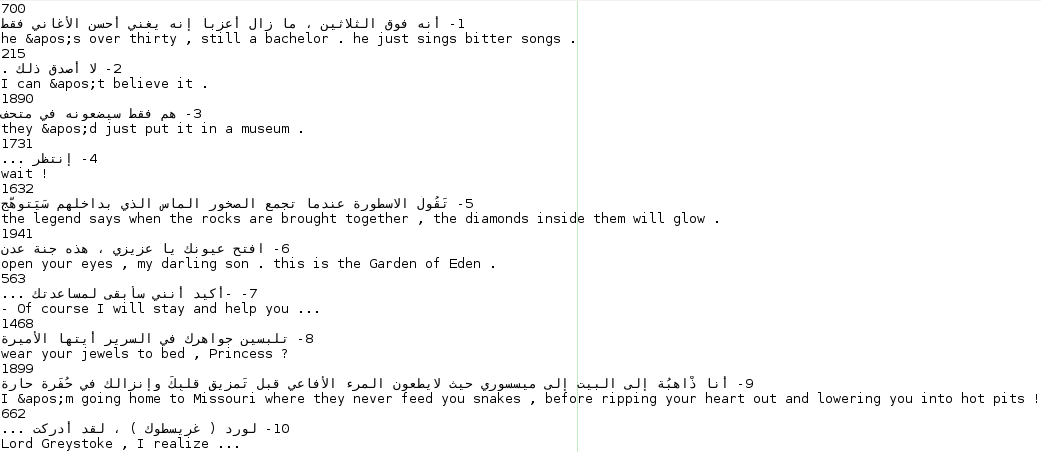
\includegraphics[scale=0.5]{randomtest.png}
\caption{the sentence number in random file, followed by Arabic sentence (right to left) starting with sentence number (1 to 10) followed by the english sentence.(left to right)\label{fig:1}}
\end{figure}
\section{Notes on the original translation}
\begin{itemize}
\item I would say the translation it self is not accurate in sense of using different expresion (using best instead of better) and in sense of the using mix of accents with standard accent.
\item The translation it self is not the best form that I would use to translate those seneteces.
\item diaractecs is also included in some cases (removing them lead to lose of meaning in some cases).
\end{itemize}
\section{Baseline}
For the baseline (used the previous bash code exactly) I got the following score\footnote{The best score between all the 3 tuning operations} score:\\ \texttt{BLEU = 24.23, 57.5/31.8/19.5/12.1 (BP=0.945, ratio=0.946, hyp\_len=13502, ref\_len=14266)}\\
Figure \ref{fig:2} show the baseline translation.
\begin{figure}[H]
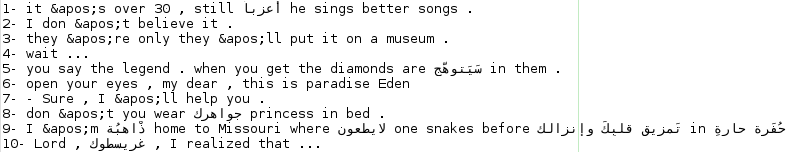
\includegraphics[scale=0.5]{baselinetest.png}
\caption{baseline translation with id\label{fig:2}}
\end{figure}
\section{Compund Split}
For this method I used the bash code \href{https://github.com/aqeel13932/MT/blob/master/03PreProcessing/CompoundSplitter.sh}{here}. The best score was :\\ \
\texttt{BLEU = 23.81, 57.6/31.8/19.3/11.9 (BP=0.934, ratio=0.936, hyp\_len=13359, ref\_len=14266)}\\ The output for the same sentences where as shown in Figure 3 \ref{fig:3}
\begin{figure}[H]
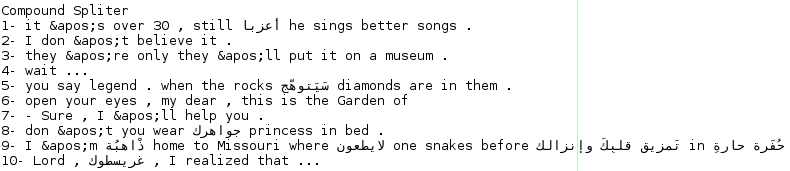
\includegraphics[scale=0.5]{compoundsplitter.png}
\caption{compound splitter translation with id\label{fig:3}}
\end{figure}
\section{Byte Pair Encoding}
After 26 hours of computation time I found that it has a bug with arabic language (instead of output like \texttt{a@@} \(\rightarrow\) \texttt{a @ @})
\section{Comparision}
First let's take a look at Figure \ref{fig:4} were we can see all the data in one place.
\begin{figure}[H]
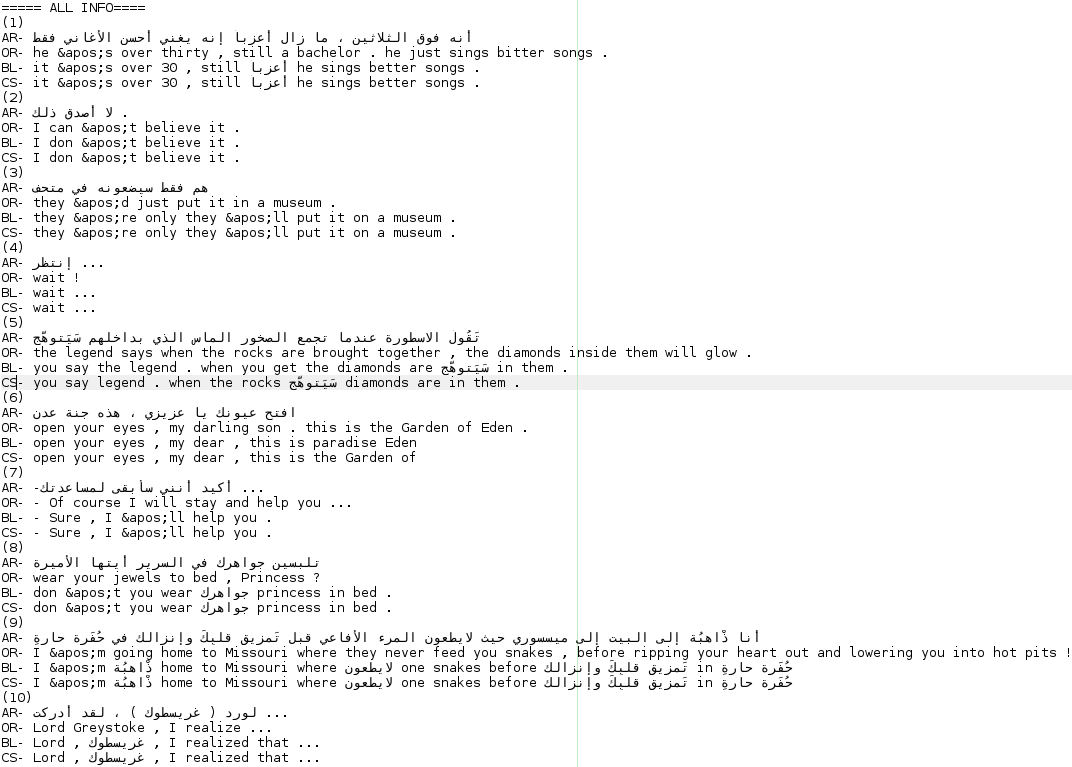
\includegraphics[scale=0.5]{All.png}
\caption{show different translation, \texttt{AR: arabic, ORG: original translation, BL: Baseline, CS: Compound splitter}\label{fig:4}}
\end{figure}
The following table show the sentences and the methods:
\begin{table}[H]
\begin{tabular}{|c|c|c|c|}
\hline
Sentence ID& Baseline & Compound Split &Notes\\
\hline
1&same&same& Considered the error bitter and (it's instead of he) to equalize them\\
\hline
2&better&better&\\
\hline
3&worse&worse&\\
\hline
4&same&same&\\
\hline
5&worse&worse&\\
\hline
6&Better&Worse\\
\hline
7&worse&worse& Even the original one is not that good :( \\
\hline
8&worse&worse&\\
\hline
9&worse&worse& (there is a typo in the original translation)\\
\hline
10&same&same& equalized the untranslated word with catching the right sentence time (past) \\
\hline
\end{tabular}
\end{table}
\section{Comments}
I would like to comment the following points :
\begin{itemize}
\item Using compound split didn't improve the performance. The result wasn't shocking since arabic language don't have much of long words ( can't think of any long words like german words) unless we include the diaractects ( which I suspect to be the difference between the baseline and compound splitter way).
\item Looking at the random results I found problems in English subtitles and Arabic subtitles as well.
\item The data mainly was English to Arabic but I used it in reverse. So I considered the Arabic text as the original and I liked that at some points the models performed better than the original English text in catching the sentence time.
\item In the data there were some typos which popup the problem of unseen words.
\end{itemize}
\section{Acknowledgement}
Thanks to Hasan helped me to recognize the error when merging \texttt{migiza} with \texttt{moses}.\\
Thanks to Maksym, told me about \texttt{cmph} library which without it my laptop won't handle all this data.\\
\textbf{Please Note:} All tex,pdf,.sh,... files exist on \href{https://github.com/aqeel13932/MT/tree/master/03PreProcessing}{github}

{\center \textbf{E.O.F\\}}

\end{document}